\begin{figure}[H]
  \centering
  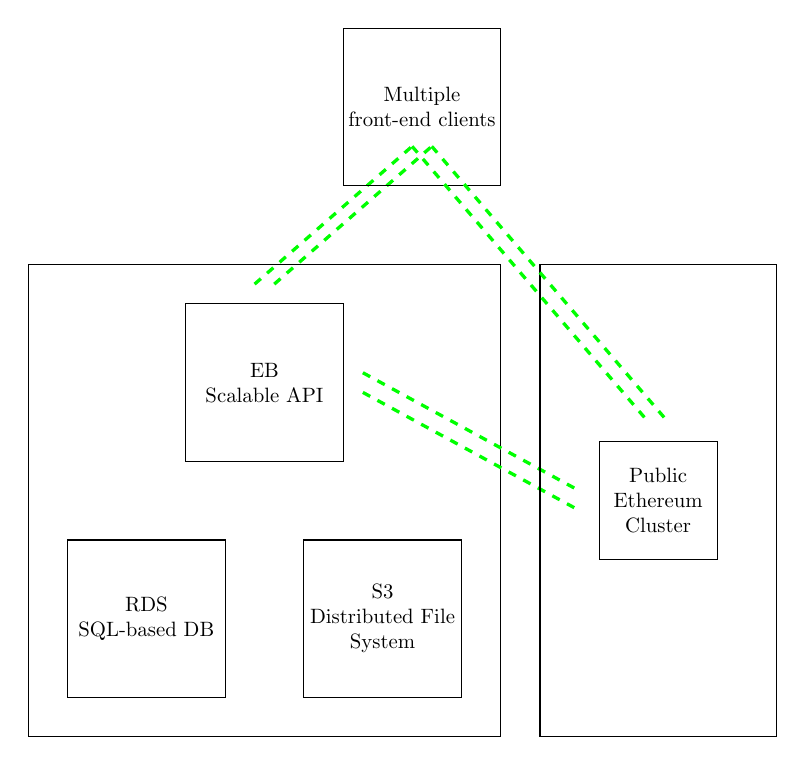
\begin{tikzpicture}[scale = 0.5, every node/.style={scale = 0.75}]

  % AWS Architecture
  \draw (-1, -1) rectangle (11, 11);
  \draw (0, 0) rectangle (4, 4);
  \draw (6, 0) rectangle (10, 4);
  \draw (3, 6) rectangle (7, 10);
  \draw[dashed, very thick, green] (4.75, 10.5) -- (8.75, 14);
  \draw[dashed, very thick, green] (5.25, 10.5) -- (9.25, 14);
  \draw[dashed, very thick, green] (7.5, 8.25) -- (13, 5.25);
  \draw[dashed, very thick, green] (7.5, 7.75) -- (13, 4.75);

  % Ethereum
  \draw (12, -1) rectangle (18, 11);
  \draw (13.5,  3.5) rectangle (16.5, 6.5);

  % Front-end services
  \draw (7, 13) rectangle (11, 17);
  \draw[dashed, very thick, green] (8.75, 14) -- (14.75, 7);
  \draw[dashed, very thick, green] (9.25, 14) -- (15.25, 7);

  \node[align=center] at (2, 2) { RDS\\SQL-based DB };
  \node[align=center] at (8, 2) { S3\\Distributed File\\System };
  \node[align=center] at (5, 8) { EB\\Scalable API };
  
  \node[align=center] at (9, 15) { Multiple\\front-end clients };
  
  \node[align=center] at (15, 5) { Public\\Ethereum\\Cluster };

  \end{tikzpicture}
  \caption{
    Potential architecture for proof of concept. Shows links between different systems using green, dashed lines. Each inner box referring to a specific service within a location (public or private). All links are made over public infrastructure.\textit{The Electron application that will be built as part of this proof of concept is assumed to be one of many front-end clients.}
  }
  \label{fig:arch_potential_1}
\end{figure}


